\documentclass[10pt,a4paper]{article}
\usepackage[utf8]{inputenc}
\usepackage[italian]{babel}
\usepackage{amsmath}
\usepackage{amsfonts}
\usepackage{amssymb}
\usepackage{graphicx}
\author{Danilo ``Bestbug'' Giordani}
\title{Appunti crittografia I}


\begin{document}
\maketitle
\section{Prefazione}
La crittografia è lo studio e progettazione di algoritmi , assieme alla crittoanalisi (studio della forza di un crifrario) forma la crittologia. La crittografia fa parte della teoria dei codici: tecniche utilizzate per trasmettere e memorizzare le informazioni su un canale rumoroso. Nello specifico la crittografia dice come rendere sicuro questo canale. Nelle analisi che andremmo a fare sui vari cifrari avremo una situazione in cui alice e bob cercano di comunicarsi un messaggio mentre eva vuole impossersarsi del messaggio.

\begin{figure}[htbp]
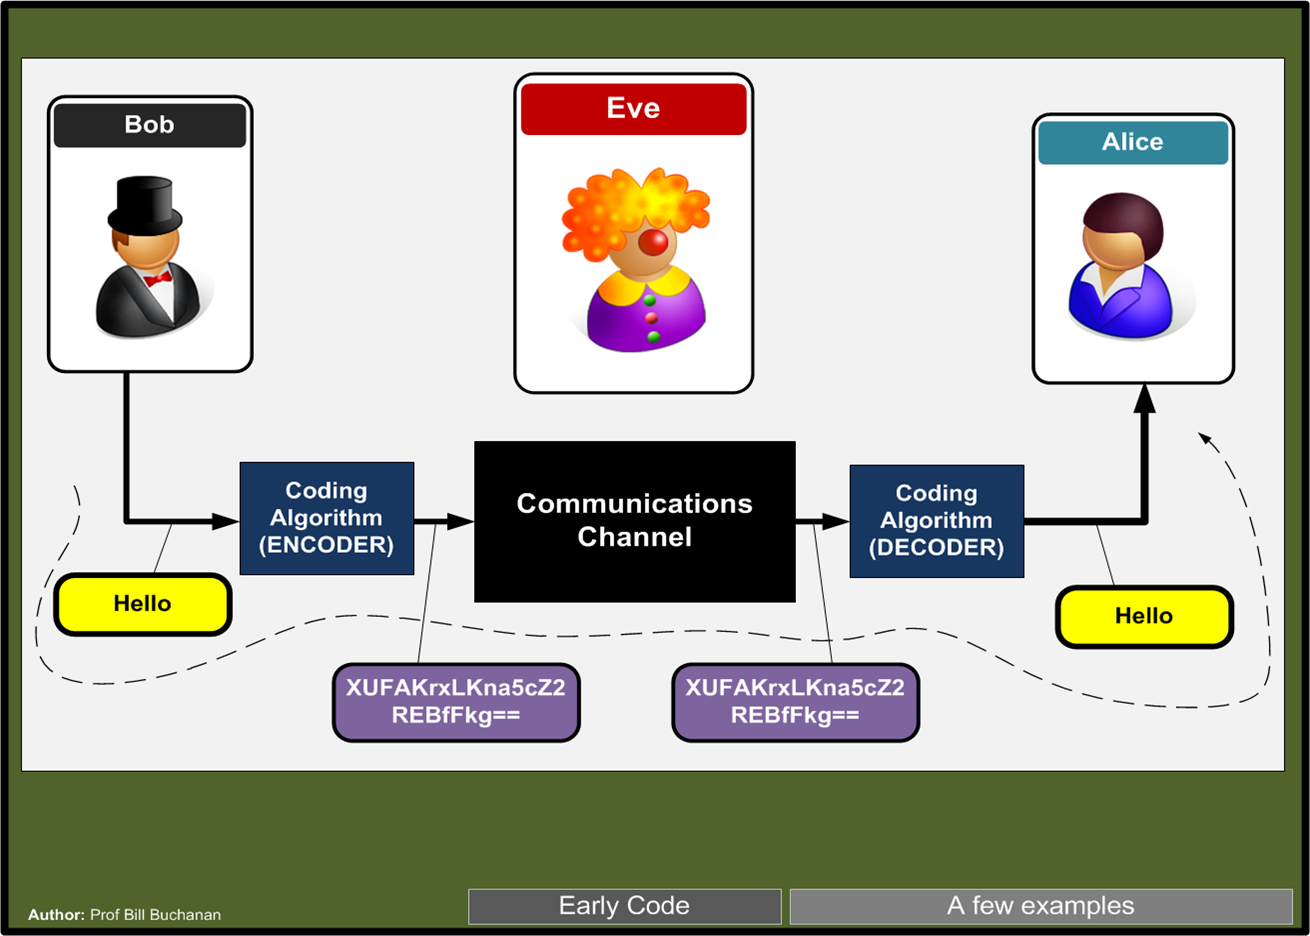
\includegraphics[scale=0.4]{immagini/eve1.png}
\end{figure}

\subsection{Principio di Kerkof (1800)}
 ``l'attaccante sa tutto tranne la chiave e il contenuto del messaggio.''\\
Questo principio vuole far notare che un cifrario è forte solo se non usa dati al di fuori della chiave per crittare il messaggio. Si predilige inoltre un cifrario aperto in modo che si possa analizzare e capire se e dove ci sono le debolezze

\subsection{Modalità di attacco}
Eva generalmente ha 4 modalità di attacco:\\
\begin{itemize}
\item Ciphertex only: eva ha solo il testo cifrato e prova a decifrarlo fino ad ottenere un testo sensato
\item Known plaintext: eva ha il plaintext e il suo testo cifrato
\item Choosen plaintext: eva sceglie che info cifrare in modo da cercare casi particolari
\item Choosen Ciphertex: eva può decifrare del testo inventato da lei in cerca di casi particolari
\end{itemize}
\subsection{Tipi di cifrari}
Prima del 1970 esistono 2 tipi di cifrari simmetrici e la steganografia, successivamente nascono i cifrari asimmetrici. Questi ultimi sono meno veloci rispetto a quelli simmetrici. Un metro di valutazione efficace per valutare un cifrario è la sua resistenza all'attacco di tipo forza bruta (provando tutte le combinazioni possibili quanto ci metto mediamente ad "indovinare" la chiave?). La soluzione possibile per risolvere questo attacco è di aumentare la chiave per multipli di 8 bit.

\section{cifrari storici}
\subsection{cifrari monoalfabetici a sostituzione}
\subsubsection{Cifrario di Cesare}
Si prende un valore x e si aggiunge un valore K il risultato, che indichiamo con y, è il testo cifrato:
\begin{center}
$y=(x+k)\mod26$
\end{center}
Vediamo ora come si può attaccare questo cifrario:\\
\textbf{Attacco Ciphertex only}: provo tutti i K fino a quando non riesco ad ottenere un plaintext sensato
\textbf{Attacco known plaintext}: sapendo che la lettera 't' è stata codificata con 'd' e sapendo che 't' è 19 e 'd' è 3 posso ottenere k:\\
$$(19+k)\mod26 = 3\mod26 \rightarrow k=10$$
\textbf{Attacco choosen plaintext}: dato che A è stato codificato con 1 cifro il testo 'A' e ottengo direttamente la chiave
\textbf{choosen Ciphertex}: provo a decrittare 'A' e ottengo -k
\subsubsection{Quadrato di polimio}
Si tratta di un quadrato $5 \times 5$

La scacchiera originale è costituita da una griglia composta da 25 caselle ordinate in cinque righe ed altrettante colonne. Le lettere dell'alfabeto vengono inserite da sinistra a destra e dall'alto in basso. Le righe e le colonne sono numerate: tali numeri sono gli indici o "coordinate" delle lettere costituenti il messaggio in chiaro:
\begin{center}
\begin{tabular}{c|c|c|c|c|c|}
 & 1& 	2& 	3& 	4& 	5\\
 \hline
 1& 	A& 	B& 	C& 	D& 	E\\
 2& 	F& 	G& 	H& 	I, J& 	K\\
3& 	L& 	M& 	N& 	O& 	P\\
4& 	Q& 	R& 	S& 	T& 	U\\
5& 	V& 	W& 	X& 	Y& 	Z\\
\end{tabular}
\end{center}



La trasposizione avviene sostituendo ad ogni lettera del messaggio un numero le cui cifre rappresentano il numero di riga e di colonna della sua posizione nella scacchiera. Ad esempio, operando sulla parola "WIKIPEDIA":\\

    la lettera "W" si trova nella 5ª riga e 2ª colonna, per cui il suo codice sarà 52;\\
    la lettera "I" si trova sulla 2ª riga e 4ª colonna, per cui il suo codice sarà 24;\\

Proseguendo con questo metodo il risultato finale per "WIKIPEDIA" sarà « 52 24 25 24 35 15 14 24 11 ».
\subsection{Cifrario affini}
Risulta molto simile a cesare solo che lo zero non si trova in 0 ma in q:

$$y=(mx+q)\mod26$$

Esempio: $y=9\cdot7+2\mod26 \leftarrow13$
Risulta quindi necesaria l'esistenza dell'\textbf{inverso moltiplicativo} in $Z_n$. Questa condizione è "gratis" se si lavora in un campo (con n numero primo) dove ho sempre l'inverso, se si lavora in un anello infatti non è detto che l'inverso esista sempre. Esiste una CNS se non si vuole usare un campo: se n e x sono coprimi (ovvero MCD(n,x)=1), dato che solitamente un campo $Z_n$ n è primo questa condizione è sempre verificata.
L'esempio precedente decifro y nel seguente modo:

$$x=\frac{1}{9}\cdot(y-2)\mod26$$
$$x=3\cdot(y-2)\mod26$$
$$x=7$$

l'inverso di $\frac{1}{9}$ lo si ottiene nel seguente modo:
$$9\cdot=1\mod26$$
$$x=3$$

\textbf{Attacco know plaintext} \\
Sappiamo che if(8,5)$\rightarrow$pq(15,16) allora:\\
$
\begin{cases}
15=8\cdot k+h \mod 26 \\
16 = 5\cdot k+h \mod26
\end{cases}
\rightarrow
\begin{cases}
k=17\\
h=9
\end{cases}
$
\newpage
\subsubsection{Problema analisi delle frequenze per i cifrari affini}
In questo tipo di cifrario si sfrutta la debolezza dell'alfabeto di riferimento (sappiamo che alcune lettere si ripetono con più frequenza se il plaintext è in italiano rispetto allo stesso plaintext di riferimento)
\begin{figure}[htbp]
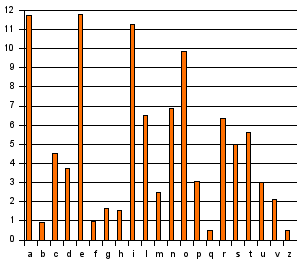
\includegraphics[scale=0.8]{immagini/Frequenze-alf_it.png}
\caption{frequenze delle lettere nell'alfabeto italiano}
\end{figure}

\subsection{Polialfabetici a sostituzione}
Risolvono il problema delle analisi delle frequenze facendo uso di un numero più o meno grande di alfabeti per sostituire le lettere del messaggio, usando un determinato ordine che costituisce la chiave. Esempio di cifrario polialfabetico è il cifrario di Vigenere. Si contrappone ai cifrari a sostituzione di tipo monoalfabetico quale ad esempio il cifrario di Cesare.

\subsubsection{Cifrario di Vigenere}
Il metodo si può considerare una generalizzazione del cifrario di Cesare; invece di spostare sempre dello stesso numero di posti la lettera da cifrare, questa viene spostata di un numero di posti variabile ma ripetuto, determinato in base ad una parola chiave, da concordarsi tra mittente e destinatario, e da scrivere ripetutamente sotto il messaggio, carattere per carattere; la chiave era detta anche verme, per il motivo che, essendo in genere molto più corta del messaggio, deve essere ripetuta molte volte sotto questo, come nel seguente esempio:\\
\begin{center}
\begin{tabular}{ll}
Testo chiaro &- RAPPORTOIMMEDIATO\\
Verme &- VERMEVERMEVERMEVE\\
Testo cifrato &- MEGBSMXFUQHIUUEOS\\
\end{tabular}
\end{center}
Il testo cifrato si ottiene spostando la lettera chiara di un numero fisso di caratteri, pari al numero ordinale della lettera corrispondente del verme. Di fatto si esegue una somma aritmetica tra l'ordinale del chiaro (A = 0, B = 1, C = 2...) e quello del verme; se si supera l'ultima lettera, la Z, si ricomincia dalla A.

\subsubsection{Debolezza del Cifrario di Vigenere: l'attacco di Kasinski}
Sfrutta l'attacco delle analisi delle frequenze dividendo il testo cifrato in n sottoistanze. Per far ciò si possono utilizzare metodi statistici per trovare n, e successivamente applicare l'analisi delle frequenze a ciascun alfabeto cifrante. Ovvero, se abbiamo come chiave VERME, basta operare l'analisi delle frequenze per tutte le lettere crittate dalla V, poi per quelle crittate dalla E, ecc. Perciò, la prima, la sesta, l'undicesima, ecc. lettera avranno lo stesso alfabeto cifrante. La parte più complicata sta dunque nello scoprire la lunghezza della chiave cifrante anche se la cosa non è impossibile. Nel testo cifrato infatti, se la chiave utilizzata è breve, vi saranno probabilmente delle serie di lettere ripetute. Queste serie di lettere, se abbastanza lunghe (5-6 caratteri), saranno generate probabilmente dalla stessa parola in chiaro. Basterà allora calcolare la distanza tra una parola e l'altra e la lunghezza della ripetizione per risalire alla lunghezza n della chiave. Così facendo si può capire quali lettere usano il primo alfabeto cifrante, quali il secondo, e così via procedendo poi con l'analisi delle frequenze per ciascun alfabeto.

\subsubsection{Cifrario di Gardano}
Risulta essere come Vigenere solo che la chiave è formata da chiave+plaintext. Ha come vantaggio una maggiore resistenza all'attacco di Kasinski

\subsubsection{Cifrario Playfair}
La tecnica cifra coppie di lettere (digrafi), invece che una singola lettera come nel semplice cifrario a sostituzione di Vigenère allora in uso. Playfair è quindi significativamente più difficile da forzare poiché l'analisi delle frequenze usata per i semplici cifrari a sostituzione non funzionano con esso. L'analisi delle frequenze può essere ancora intrapreso, ma sono possibili 600 digrafi [1] invece di 26 monografi. L'analisi della frequenza dei digrafi è possibile, ma considerevolmente più difficile. Inoltre le frequenze relative delle singole lettere hanno un intervallo molto più ampio di quello dei digrafi, rendendo l’analisi delle frequenze ulteriormente complicata. Per questi motivi, a suo tempo, il codice Playfair era considerato inviolabile.

\subsubsection{cifrario ADFGX}

Nella primavera del 1918 le truppe tedesche stavano pianificando una serie di attacchi in forze per sfondare le linee nemiche (Offensive di primavera) e dirigersi verso Parigi. Per rendere sicura la trasmissione dei piani di attacco alle truppe fu deciso di cifrare le comunicazioni mediante l'uso di un cifrario inventato dal colonnello Nebel denominato ADFGX, dalle uniche lettere che apparivano nel testo cifrato (in alcune versioni venivano usate le lettere ADFMX); tale cifrario derivava da un precedente schema crittografico noto come GEDEFU 18 (GEheimschrift DEr FUnker 18, o cifrario dei radiotelegrafisti 18). Le lettere del testo cifrato venivano selezionate da una scacchiera di dimensioni 5x5 (quindi con 25 possibili combinazioni) con l'unica differenza rispetto agli altri cifrari a trasposizione che per gli indici delle righe e delle colonne non erano usati numeri ma lettere (A, D, F, G e X, appunto). Essendo le possibili combinazioni solo 25, le 26 lettere dell'alfabeto non rientravano nello schema per cui fu scelto di cifrare le lettere "I" e "J" con lo stesso simbolo. La disposizione delle lettere nella scacchiera era data da una chiave che cambiava quotidianamente.

\subsection{cifrari a blocchi}
\subsubsection{cifrario di Hill (1929)}
È il primo cifrario che introduce l'algebra lineare e modulare.\\
Nella cifratura, ogni lettera è per prima cosa codificata in numero. Lo schema usato più di frequente è semplicemente: A = 0, B = 1, ..., Z = 25, ma questa non è una caratteristica essenziale del cifrario. Un blocco n di lettere è quindi considerato come uno spazio vettoriale di dimensione n, e moltiplicato per una matrice n x n, modulo 26 (se si usa un numero più alto di 26 nel modulo base, allora si può usare uno schema numerale diverso per codificare le lettere, ed è possibile anche utilizzare spazi e punteggiatura). L'intera matrice è considerata la chiave del cifrario e deve essere casuale, a patto che sia invertibile in $\mathbb{Z}_{26}^n$ (per assicurare che la decrittazione sia possibile). Considerando il messaggio 'TUO' e la seguente chiave (che in lettere sarebbe Y Y P R Z W I Z J):

    $$\begin{pmatrix} 24 & 24 & 15 \\ 17 & 25 & 22 \\ 08 & 25 & 09 \end{pmatrix} $$

Considerando che ‘T’ è ‘19’, ‘U’ è ‘20’ e ‘O’ è ‘14’, il messaggio è il vettore:

   $$ \begin{pmatrix} 19 \\ 20 \\ 14 \end{pmatrix}$$

Conseguentemente il vettore cifrato è dato da:

    $$\begin{pmatrix} 24 & 24 & 15 \\ 17 & 25 & 22 \\ 08 & 25 & 09 \end{pmatrix} \begin{pmatrix} 19 \\ 20 \\ 14 \end{pmatrix} = \begin{pmatrix} 1146 \\ 1131 \\ 778 \end{pmatrix} \pmod{26} \equiv \begin{pmatrix} 02 \\ 13 \\ 24 \end{pmatrix} $$

che corrisponde al testo crittato ‘CNY’.\\
Il calcolo è dato dalla moltiplicazione matrice $\times$ testo in chiaro. Dopo aver effettuato questo calcolo, al risultato si toglie il modulo (in questo caso 26) tante volte quante ne servono per avere come differenza un numero inferiore del modulo stesso e che dia, quindi, in risultato una lettera ben definita.

    $$C \leftarrow 02 = 24 \cdot 19 + 24 \cdot 20 + 15 \cdot 14 \pmod{26}$$
    $$N \leftarrow 13 = 17 \cdot 19 + 25 \cdot 20 + 22 \cdot 14 \pmod{26}$$
    $$Y \leftarrow 24 = 08 \cdot 19 + 25 \cdot 20 + 09 \cdot 14 \pmod{26}$$
    
Come si può notare la matematica dietro questo cifrario inizia a diventare complessa anche su esempi semplici.

\subsubsection{Proprietà dei cifrari a blocchi}
Nel 1950 Cloude Channon afferma che i codici devono avere 2 proprietà:
\begin{itemize}
\item Con una piccola modifica in input si deve generare una grossa variazione in output (proprietà di confusion)
\item Nel cipertext un singolo carattere deve dipendere da più carattere in input (proprietà di diffusion)
\end{itemize}
l'esempio principe di queste due proprietà è otp
\subsubsection{One Time Pad (OTP)}
In questo cifrario la chiave è una stringa pseudo casuale (quindi non predicibile) lunga quanto il plaintext che si usa per xorare bit a bit il plaintext rendendo quindi un cipertext unico. Questo è l'unico cifrario considerato sicuro ma il suo limite è come gestire la chiave dato che risulta essere lunga, difficile da spedire e generare. Esiste un metodo migliore? Si con le funzioni one way è facile arrivare nel codominio ma è difficile tornare nel dominio inziale.

Esempio:
$x_j=x^2_{j-1}\mod n$

Dove il risultato finale è formato dai bit meno significativi del risltato della potenza.
\subsubsection{linear feedback shift register (LFSR)} 
Gli LFSR possono essere implementati in hardware, e ciò li rende utili in applicazioni che richiedono la generazione molto rapida di numeri pseudo-casuali, come nella tecnica radio Direct Sequence Spread Spectrum, usata ad esempio nell'UMTS.

Il Global Positioning System (GPS) usa gli LFSR per trasmettere rapidamente una sequenza che indica degli istanti relativi ad alta precisione, sfruttandone il determinismo: basta infatti trasmettere il seme utilizzato nel trasmettitore e la sequenza generata sarà identica anche sul ricevitore.

\section{Problemi difficilmente risolubili}
Come vedremo prossimamente i cifrari moderni sono considerati sicuri non quanto per la complessità delle loro operazioni ma dalla difficoltà di fattorizzare (trovare i numeri primi il cui prodotto forma il numero) i numeri "grandi" in poco tempo. Vediamo ora alcuni teoremi a riguardo.

\subsection{Teorema dei numeri primi}
Se $\pi(x)$ è il numero di numeri primi minori di x allora:
$$\pi(x) \sim \frac{x}{\log x}$$
Ovvero che ci sono ``tanti'' numeri primi
\begin{itemize}
\item Ogni intero positivo è prodotto di numeri primi, questa fattorizazione è unica a meno dell'ordine dei fattori
\item Si usa l'algoritmo di euclide: il resto che precede lo 0 è il MCD(a,b)
\end{itemize}
Esempio:\\
$\text{MCD} (1180,482) \rightarrow
1180 = 2 \cdot 482+216 \rightarrow
482 = 2 \cdot 216+50 \rightarrow
216 = 4 \cdot 50+16 \rightarrow
50 = 3 \cdot 16+2 \rightarrow
16 = 8 \cdot 2 +0$\\
\textbf{Vantaggi}:
\begin{itemize}
\item Non richiede la fattorizzazione dei numeri primi
\item È veloce
\end{itemize}

\subsection{Proprietà delle congruenze}
Siano a,b due interi non nulli e sia d=mcd(a,b) allora esistono due interi x e y tc $ax+by=d$. In particolare se a e b sono primi tra loro allora esistono due interi x e y tc $ax+by=1$

\subsection{Algoritmo di Euclide esteso}
Precondizione:\\
Se MCD(a,n)=1 $\exists$ inverso
$a \cdot s+n \cdot t = 1 \mod n$\\
$a \cdot s \equiv 1 \mod n$

\subsection{Teorema cinese dei resti}
Si usa il teorema cinese dei resti per velocizare i conti in modulo. Serve per spezzare una congruenza $\mod (n)$ in un sistema di congruenze in $\mod(fattori di n)$.
\textbf{definizione}: siano m ed n due interi positivi tc $mdc(m,n)=1$ dati a,b interi $\exists$ soluzione x(con $\! \! \! \mod(m\cdot n)$) del sistema di congruenze:

$\begin{cases}
x \equiv a \mod(n) \\
x \equiv b \mod(m)
\end{cases}$

Esempio:\\
$
p= r_1 \cdot r_2 \cdot r_3 \cdot ... \cdot r_n \\
p_i=\frac{P}{r_i} \\
q_i=p_i^{-1} \mod r_i\\
x \equiv pippo \mod p \Rightarrow
\begin{cases}
x=a_1 \cdot \mod r_1 \\
x=a_2 \cdot \mod r_2 \\
x=a_3 \cdot \mod r_3 \\
. \\
. \\
. \\
x=a_n \cdot \mod r_n
\end{cases}
\Rightarrow x= \sum\limits_{i=1}^{n} a_i \cdot p_i \cdot q_i \mod p
$
\subsection{Teorema di fermat}
$a^{p-1} \equiv 1 \mod p$ Se p è primo e a qualsiasi \\
\textbf{teorema di eulero-fermat}\\
$a^{\phi(1)} \equiv 1 \mod p$ se MCD(a,n)=1 con a qualsiasi e n qualsiasi
\textbf{Funzione di Eulero}\\
Dato n:\\
\begin{itemize}
\item se è primo $\phi(n) = n-1$
\item se è composizione di due primi allora $p \cdot q \Rightarrow \phi(n)= (p-1)\cdot (q-1)$
\item se è composizione di più di due primi allora $\phi(n) = n \cdot \pi(1-\frac{1}{p}) $
\end{itemize}
\section{Cifrari a chiave asimmetrica}
\subsection{Prefazione}
Nati nel 1970 nascono i cifrari con chiave asimmetrica, che dove ci si ritrova per la prima volta con due chiavi: una pubblica che consegnero ad alice per cifrare il messaggio e una privata che la userò per decifrare il messaggio. Idealmente:
\begin{itemize}
\item Alice chiede a Bob di spedirle il suo lucchetto, già aperto. La chiave dello stesso verrà però gelosamente conservata da Bob.
\item Alice riceve il lucchetto e, con esso, chiude il pacco e lo spedisce a Bob.
\item Bob riceve il pacco e può aprirlo con la chiave di cui è l'unico proprietario.
\end{itemize}

\begin{figure}[htbp]
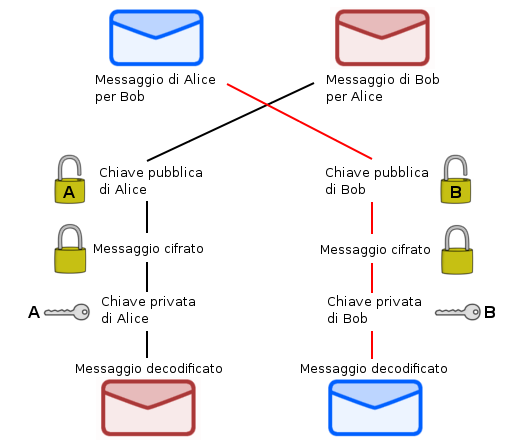
\includegraphics[scale=0.4]{immagini/Crittografia_asimmetrica_schema.png}
\end{figure}

Un'altro vantaggio di usare la crittografia asimetrica è la riduzione del numero di chiavi, vediamolo con un esempio:\\

Se 10 persone volessero comunicare in maniera simmetrica ho $\binom{10}{2} = 45$ chiavi. Nel caso assimetrico invece ho solo 20 chiavi. Le chiavi sono di meno nel caso di grandi numeri mentre con piccoli numeri risultano essere di meno quello simmetriche. Con i cifrari asimmetrici il ciphertext è computazionalmente intrattabile.
\subsection{RSA}
Il funzionamento di RSA è molto semplice: basta infatti eseguire una potenza in modulo. Vediamo ora i passi nel dettaglio
\subsubsection{Generazione della chiave}
La generazione delle due chiavi si divide in 5 parti:
\begin{itemize}
\item Scegli due primi $p$ e $q$ primi molto grandi (almeno 1024 bit) in maniera casuale
\item Calcola il valore n tc $n = p \cdot q$
\item Calcola $\phi(n) = \phi(p) \cdot \phi(q) = (p - 1)(q - 1) = n - (p + q -1)$ (dove $\phi$ è la funzione di eulero)
\item Scegli un valore $1<e<\phi(n)$ tc MCD$(e, \phi(n))=1 \Rightarrow$ MCD$(e,(p-1)\cdot(q-1))$
\item Calcola d tc $d \equiv e^{-1} \mod (\phi(n))$
\end{itemize}

Alla fine di questo procedimento abbiamo le due chiavi, quella pubblica è formata dalla coppia (n,e) mentre quella privata dalla terna (p,q,d)

\subsubsection{Come funziona RSA nella pratica}
Cifratura:\\
ciphertext = $plaintext^e \mod(n)$\\
Decifratura:\\
plaintext: $ciphertext^d \mod(n)$\\ \\
Esempio:\\
plaintext = 88, $K_pubblica(187,7), K_privata(p,q,d)$
ciphertext: $88^7 \mod(187) \Rightarrow 11$\\
plaintext: $11^23 \mod(187) \Rightarrow 88$\\
Bisogna fare attenzione che il messaggio deve essere al più uguale alla dimensione $n$ se il messaggio è di dimensione più grande si divide in ``parti'' che hanno dimensione $n$

\subsubsection{Dimostrazione corettezza RSA}

Siano $p,q$ primi tc $MCD(e,\phi(n))=1$ e:\\
$e\cdot d \equiv 1 \mod(\phi(n))$\\
$ciphertext: plaintext^e \mod(n)$\\
$plaintext: ciphertext^d \mod(n)$\\
Allora possiamo dire che:
$(ciphertext)^d \mod(n) \equiv ((plaintext)^e)^d \mod(n) \equiv plaintext^{e\cdot d} \mod(n)$\\
Vogliamo ora riscrivere $e \cdot d$ in una maniera più comoda, sfruttiamo quindi la funzione di Eulero tenendo a mente 3 cose:\\
\begin{itemize}
\item[1)]$\phi(n) = \phi(p\cdot q) = (p-1)\cdot(q-1)$
\item[2)]$e\cdot d = 1 \cdot \mod(\phi(n))$
\item[3)]$e\cdot d = 1 \cdot K\cdot \phi(n)$
\end{itemize}
Riscriviamo ora $e \cdot d$:\\
$(plaintext)^{K \cdot \phi(n)+1}\mod(n) = (plaintext)^{k\cdot(p-1)\cdot(q-1)+1}\mod(n)\equiv plaintext$\\
Dimostriamo ora che quanto scritto è corretto, semplifichiamo la dimostrazione e spezziamola in 3 parti: la prima parte dimostriamo per p la seconda parte per q ed infine per $p\cdot q$:\\
$(plaintext)^{k\cdot(p-1)\cdot(q-1)+1}\mod(n)=m$ sfrutto il teorema cinese dei resti:\\
$m\mod(q\cdot p) \Rightarrow \begin{cases}a\mod p \\b\mod q\end{cases}$

divido quindi l'ipotesi in due parti:
\begin{center}
$\begin{cases}
(m)^{k\cdot(p-1)\cdot(q-1)+1}\mod(p)\equiv m \mod(p) (1)\\
(m)^{k\cdot(p-1)\cdot(q-1)+1}\mod(q)\equiv m \mod(q) (2)
\end{cases}
$\\
\end{center}

Iniziamo a dimostrare la prima congruenza:\\
Ci sono due casi:
\begin{center}
$\begin{cases}
MCD(p,m)\not=1\\
MCD(p,m)=1
\end{cases}
$\\
\end{center}
Se siamo nel primo caso p e m non sono coprimi ma dato che p è primo allora sicuramente m è un multiplo di p quindi:\\
$m\equiv 0 \mod(p) \Rightarrow (m)^{k\cdot(p-1)\cdot(q-1)+1}\mod(p)\equiv m \mod(p)  \forall e,d$\\
Se invece siamo nel secondo caso allora:\\
$m^{(p-1)} \equiv 1 \mod(p) \Rightarrow [m^{(p-1)}]^{k\cdot (q-1)}\cdot m \mod(p) \equiv m $ Dato che 1 è l'elemento neutro della moltiplicazione (così come le sue potenze) $ \Rightarrow 1^{k\cdot (q-1)}\cdot m \mod(p) \equiv 1^{k\cdot(q-1)}\cdot m$

La seconda congruenza si risolve come la prima, e dato che anche q è primo

$$(m)^{K \cdot \phi(n)+1}\mod(n) \equiv m \mod(n) $$
$$(m)^{K \cdot \phi(n)+1} - m\mod(n) \equiv 0 \mod(n)$$
dato che il valore a sinistra è divisibile sia per q che per p $\Rightarrow \frac{(m)^{K \cdot \phi(n)+1} - m}{p\cdot q}$

\subsubsection{Attacchi ad RSA}
\begin{itemize}
\item se l'attaccante è a conoscenza del valore $\phi(n)$ allora può ottenere $p+q$:
$$n- \phi(n)+1 = pq-(p-1)\cdot(q-1)+1 = p\cdot q - (p\cdot q-p-q+1)+1 = p+q$$\\
prendiamo ora l'equazione $x^2+b\cdot x + c = 0$ con $b=-(p+q)$ e $c=p\cdot q$ e otteniamo che:\\
$$\begin{cases}
x_1\cdot x_2 = \frac{c}{a} = c = p\cdot q = n\\
x_1+x_2 = -\frac{b}{a} = b = p+q
\end{cases}$$\\
basta quindi trovare i punti dove si annulla l'equazione per trovare p e q.\\
Esempio:
$n=221 \phi(n)=192 \\ n-\phi(n)+1=30 \\ x^2-30\cdot x + 221 = 0 \\ x_{1,2}=\frac{+\frac{30}{2}+/- \sqrt{15^2-4\cdot a \cdot c} }{1} \Rightarrow x_1=p=13,x_2=q=17$
\item Un'altro attacco si basa sul recupero parziale della chiave privata $K_p$: se su una chiave di $m$ cifre si riescono a recuperare $\frac{m}{4}$ cifre si riesce a recuperare la chiave nella sua interezza
\item attacco allo spazio delle chiavi di $d$. Se la condizione $d<\frac{1}{3}\cdot\sqrt[4]{n}$ è falsa allora si è attaccabili
\item È possibile attaccare RSA tramite la sua implementazione:\\
So che RSA generalmente viene usato per cifrare piccoli testi di $\sim$ 8 caratteri il dominio è quindi di $\sim 10^17$ ma il mio testo \textit{m} è possibile scriverlo come $m=a\cdot b$ con $a,b\le 10^9$ quindi posso lavorare su uno spazio di $10^9$. Genero ora una tabelle nel seguente modo:
\begin{center}
\begin{tabular}{c|c}
$C\cdot x^{-e} \mod(n)$& 	$y^e \mod(n)$ \\
\hline
$C\cdot 1^e \mod(n)$& 	$1^e \mod(n)$ \\
$C\cdot 2^e \mod(n)$& 	$2^e \mod(n)$ \\
.&.\\
$C\cdot i^e \mod(n)$& 	$i^e \mod(n)$  \\
.&.\\
$C\cdot (10^9)^e \mod(n)$& 	$(10^9)^e \mod(n)$ \\
\end{tabular}\\
supponiamo che nel caso $i$ il valore a destra e sinistra sia uguale allora possiamo dire che:
$$ C\cdot i^{-e} \mod(n)=i^e \mod(n)$$
$$ C=i^e\cdot i^e \mod n$$
$$ C=(i\cdot i)^e \mod n$$\\
Ma noi sappiamo che $C=m^e \mod(n)$ quindi:
$$(x\cdot y)^e \mod n = (m)^e \mod n$$
$$ i\cdot i = m$$
Per risolvere questo attacco basta aggiungere del \textit{padding} ottenuto in maniera pseudo casuale dalla funzione OAEP(Optical assimetric encryption padding)
\end{center}
\item \textit{Common module attack}: Se Bob scrive ad Alice ed a Carol scrive lo stesso messaggio usando lo stesso modulo $n$ allora Bob è attaccabile, dimostrazione:\\
$$C_1=m^{e_1} \mod(n)$$ $$ C_2=m^{e_2} \mod(n)$$\\
Per Euclide esteso sappiamo che:\\
$$r\cdot e_1+r\cdot e_2 = 1 \mod n$$\\
Teniamolo a mente e concentriamoci sui due testi cifrati $C_1$ e $C_2$:
$$(C_1)^r\cdot(C_2)^s\mod(n)$$
$$C_1^r\cdot C_2^s \mod(n)$$
$$(m^{e_1})^r\cdot (m^{e_2})^S \mod(n)$$
$$m^{e_1\cdot r + e_2\cdot s} \mod(n)$$

Per euclide esteso sappiamo che $e_1\cdot r + e_2\cdot s$ è uguale a 1 in $\mod(n)$ abbiamo ottenuto quindi il plaintext a patto di trovare $r$ e $s$. La soluzione è di mandare messaggi uguali a persone diverse usando chiavi diverse.
\item \textit{Low exsponent attack}: questo attacco si usa quando $e$ è un valore piccolo e sfrutta il teorema cinese dei resti:\\
$\begin{cases}
c_a=m^e\mod(n_a)\\
c_b=m^e\mod(n_b)\\
c_c=m^e\mod(n_c)\\
\end{cases}\Rightarrow
$
$\begin{cases}
x=c_a\mod(n_a)\\
x=c_b\mod(n_b)\\
x=c_c\mod(n_c)\\
\end{cases}\\
Q_i=P_i^{-1}\mod n_i\\
x=\sum a_i\cdot P_i \cdot Q_i \mod(P)\\
P=n_a\cdot n_b \cdot n_c
P_i=\frac{P}{n_i}\\
Esercizio:\\
e=3\\
n_a=15\\
n_b=77\\
n_c=221\\
c_a=7\\
c_b=41\\
c_c=208\\
\begin{cases}
x=7\mod(15)\\
x=41\mod(77)\\
x=208\mod(221)\\
\end{cases}\\
x=m^e \Rightarrow m=\sqrt[e]{x}\\
P=15\cdot77\cdot221=255255\\
P_a=17017 P_b=3315 P_c=1155\\
Q_a=P_a^{-1}\mod(15)\\
Q_b=P_b^{-1}\mod(77)\\
Q_c=P_c^{-1}\mod(221)\\
x=7\cdot 17017 \cdot 13 + 41\cdot 3315 \cdot58+208\cdot1155\cdot84 \mod 255255 = 2197 \Rightarrow \sqrt[3]{2197} = 13\\
P_a\cdot x_a \mod (15) = 1 \Rightarrow 7\cdot x \mod(15) \Rightarrow x_a=13\\
P_b\cdot x_b \mod (77) = 1 \Rightarrow 4\cdot x \mod(77) \Rightarrow x_b=58\\
P_c\cdot x_c \mod (221) = 1 \Rightarrow 50\cdot x \mod(221) \Rightarrow x_c=84\\
$
\item L'ultimo attacco si basa solo su quanto tempo ci si impiega a criptare, in base a questo so da quanti (e quali) bit è composta la chiave. Per risolvere questo particolare attacco si moltiplica e divide il ciphertext per una stessa quantità generata casualmente volta per volta.
\end{itemize}
\subsection{AES}
\subsubsection{Prefazione}
AES (conosciuto anche come Rijdael) è il cifrario che sostituì DES nel 2000. Vediamo ora quali sono le caratteristiche di AES:
\begin{itemize}
\item Utilizza blocchi da 128 bit
\item Ha una chiave \textit{minima} di 128 bit, la chiave di lunghezza media è di 192 bit mentre la più grande è di 256 bit
\item Il plaintext viene trattato come una matrice $4 \times 4$ 
\item Non è un cifrario a blocchi di tipo Feistell
\item Tutto il cifrario si basa su 4 operazioni: subByte,shiftRows,mixColumn e addRoundKey.
\end{itemize}
\subsubsection{Funzionamento}
Per prima cosa AES ha un passaggio iniziale: utilizando la funzione AddRoundKey Ogni byte della tabella viene combinato con la chiave di sessione, la chiave di sessione viene calcolata dal gestore delle chiavi. Successivamente per cifrare sono previsti diversi round o cicli di processamento: ogni round (fase) dell'AES (eccetto l'ultimo) consiste dei seguenti quattro passaggi:
\begin{itemize}
\item SubByte: sostituzione non lineare di tutti i byte che vengono rimpiazzati secondo una specifica tabella.
\item ShiftRows: Spostamento dei byte di un certo numero di posizioni dipendente dalla riga di appartenenza
\item MixColumns: Combinazione dei byte con un'operazione lineare, i byte vengono trattati una colonna per volta
\item AddRoundKey: Ogni byte della tabella viene combinato con la chiave di sessione, la chiave di sessione viene calcolata dal gestore delle chiavi
\end{itemize}
Il numero di round o cicli dei quattro passaggi precedenti è 10 con l'ultimo round che salta il passaggio MixColumns. Vediamo ora il loro funzionamento nello specifico
\newpage
\subsubsection{SubByte}
Nel passaggio SubBytes ogni byte della matrice viene modificato tramite la S-box a 8 bit. Questa operazione provvede a fornire la non linearità all'algoritmo. La S-box utilizzata è derivata da una funzione inversa nel campo finito GF($2^8$), conosciuta per avere delle ottime proprietà di non linearità. Per evitare un potenziale attacco basato sulle proprietà algebriche la S-box è costruita combinando la funzione inversa con una trasformazione affine invertibile. La S-box è stata scelta con cura per non possedere né punti fissi né punti fissi opposti.

\begin{figure}[htbp]
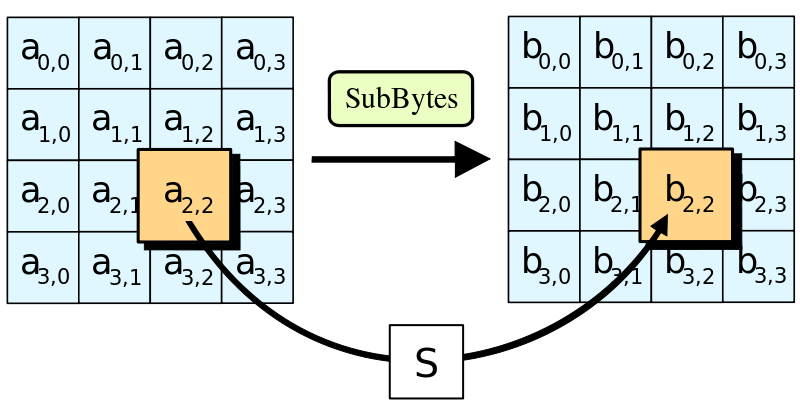
\includegraphics[scale=0.3]{immagini/SubBytes.png}
\end{figure}

\subsubsection{ShiftRows}
Il passaggio ShiftRows provvede a scostare le righe della matrice di un parametro dipendente dal numero di riga. Nell'AES la prima riga resta invariata, la seconda viene spostata di un posto verso sinistra, la terza di due posti e la quarta di tre. In questo modo l'ultima colonna dei dati in ingresso andrà a formare la diagonale della matrice in uscita. (Rijndael utilizza un disegno leggermente diverso per via delle matrici di lunghezza non fissa.)
Tutte le operazioni sono effettuate utilizzando l'indice della colonna “modulo” il numero di colonne.
\begin{figure}[htbp]
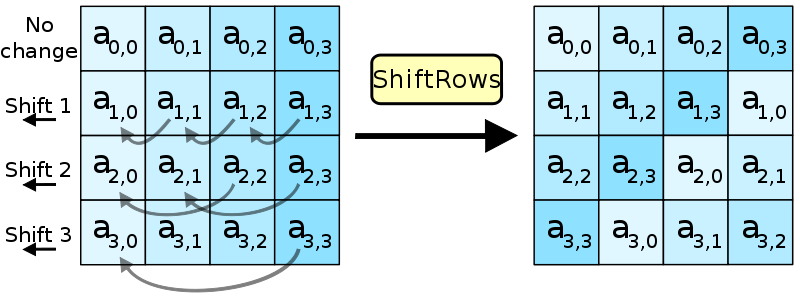
\includegraphics[scale=0.4]{immagini/ShiftRows.png}
\end{figure}

\subsubsection{MixColumns}
Il passaggio MixColumns prende i quattro byte di ogni colonna e li combina utilizzando una trasformazione lineare invertibile. Utilizzati in congiunzione, ShiftRows e MixColumns provvedono a far rispettare il criterio di confusione e diffusione nell'algoritmo (teoria di Shannon). Ogni colonna è trattata come un polinomio in GF($2^8$) e viene moltiplicata modulo $x^4+1$ per un polinomio fisso $c(x)=3x^3+x^2+x+2$.
\begin{figure}[htbp]
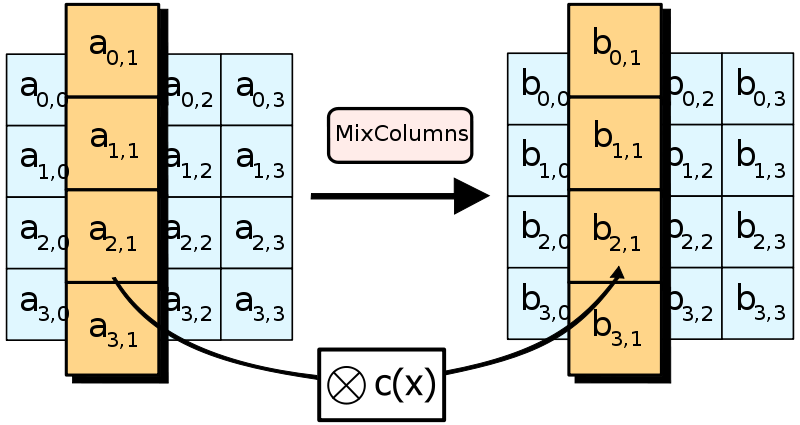
\includegraphics[scale=0.4]{immagini/MixColumns.png}
\end{figure}

\subsubsection{AddRoundKey}
Il passaggio AddRoundKey combina con uno XOR la chiave di sessione con la matrice ottenuta dai passaggi precedenti (State). Una chiave di sessione viene ricavata dalla chiave primaria ad ogni round (con dei passaggi più o meno semplici, ad esempio uno shift di posizione dei bit) grazie al Key Scheduler.
\begin{figure}[htbp]
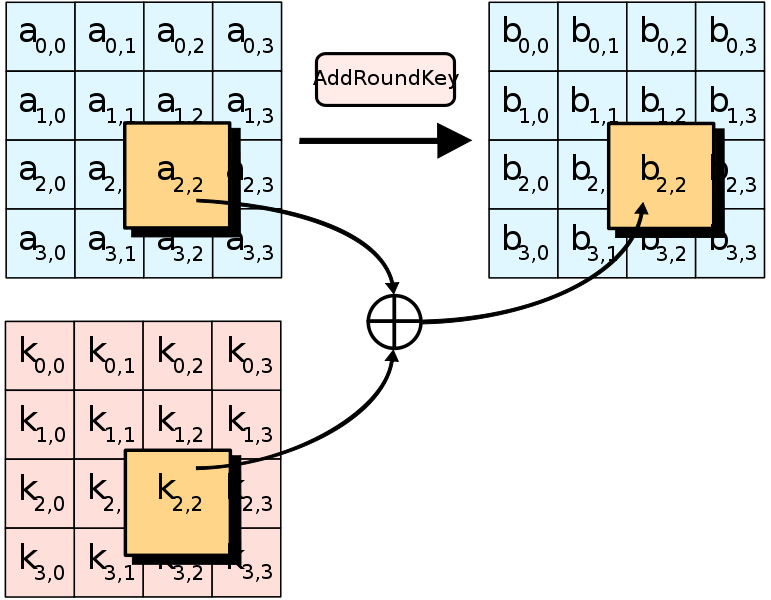
\includegraphics[scale=0.4]{immagini/AddRoundKey.png}
\end{figure}

\subsubsection{Key Scheduler}
AES (Rijndael) usa un key schedule per espandere una chiave primaria corta in un certo numero di chiavi di ciclo differenti. Questo metodo è noto con il nome key schedule di Rijndael.Il Key schedule di Rijndael utilizza un numero di operazioni comuni che vengono illustrate prima di descrivere il key schedule vero e proprio.
\subsubsection{Rotate}
L'operazione Rotate prende una parola di 32-bit come questa (in esadecimale):\\
$$1D 2C 3A 4F$$\\
e la ruota di otto bit verso sinistra, in modo che gli otto bit più a sinistra "si avvolgano" e diventino gli otto bit più a destra del risultato.\\
2C 3A 4F 1D\\

\subsubsection{Rcon}
Rcon è quello che la documentazione del Rijndael chiama l'elevamento a potenza di 2 per un valore specificato dall'utente. Quest'operazione non è eseguita sugli interi regolari, ma nel campo finito di Rijndael. In forma polinomiale, possiamo scrivere 2 come:\\
$ 2 = 00000010 = 0 x^7 + 0 x^6 + 0 x^5 + 0 x^4 + 0 x^3 + 0 x^2 + 1 x + 0 = x$, e calcolare\\
$\textrm{rcon}(i) = x^{(i-1)}$\\
in $\mathbb{F}_{2^8}$ o equivalentemente,\\
$\textrm{rcon}(i) = x^{(i-1)} \mod x^8 + x^4 + x^3 + x + 1$\\
in $\mathbb{F}_{2}[x]$.\\
Per esempio, rcon(1) = 1, rcon(2) = 2, rcon(3) = 4, e rcon(9) è il numero esadecimale 0x1b (27 in decimale).

\subsubsection{Il cuore del Key schedule}
Queste operazioni vengono utilizzate in un ciclo interno nel key schedule per generare un'array di 48 word da un byte l'una. Per fare ciò esegue i seguenti passaggi\footnote{Per maggiori informazioni si guardi il seguente link: http://www.formaestudio.com/rijndaelinspector/archivos/Rijndael\_Animation\_v4\_eng.swf }
\begin{itemize}
\item[1] si prende in input una word $W$ da 4 byte e si occupano le prime 4 posizioni dell'array
\item[2] Se si sta generando il byte in posizione $W_i$ si prende il byte in posizione $W_{i-1}$ 
\item[3] Se $W_i$ è il primo byte della chiave di round si applica la funzione Rotate definita sopra per ruotare di otto bit verso sinistra $W_{i-1}$ altrimenti si va al punto 5
\item[4] Se $W_i$ è il primo byte della chiave di round si applica la S-box di Rijndael (SubByte) su tutti e quattro i singoli byte della parola di output altrimenti si va al punto 5
\item[5] Sul primo byte della chiave di round, si applica l'OR esclusivo tra il byte, Rcon(i) e $W_{i-4}$ mentre sugli altri si applica l'OR esclusivo tra il byte, Rcon(i).
\item[6] Ogni 4 byte viene generata la chiave di round
\end{itemize}

\subsubsection{Matematica di AES}
In matematica, in particolare in algebra, un campo finito (detto a volte anche campo di Galois) è un campo che contiene un numero finito di elementi.Particolarmente utilizzati in crittografia sono i campi della forma $F_{2^n}$ poiché presentano diversi vantaggi:
\begin{itemize}
\item permettono di rappresentare univocamente ogni polinomio del campo in n bit: infatti ogni coefficiente del polinomio assumerà proprio i valori binari 0 o 1;
\item la somma tra i polinomi può essere eseguita efficientemente come semplice XOR bit-a-bit;
\item la moltiplicazione per piccoli coefficienti (1, 2 o 3) richiede al massimo uno shift a sinistra e uno XOR
\end{itemize}

\subsubsection{Decriptazione}
Il processo è molto semplice: basta infatti eseguire i round dal decimo fino al primo per riottenere il testo in chiaro

\section{Test di primalità}
\subsection{Prefazione}
Sono test probabilistici che permettono di dire se un numero n è \textit{probabilmente} primo. Questi test non fattorizzano ma trovano un contro esempio per dimostrare che è primo, il fatto che non lo riescano a dimostrare non implica che un numero n non è sicuramente primo.

\subsection{Basic priciple}
Se $n$ è un numero primo allora $\not \exists x,y$ tc:
$$x^2\equiv y^2 \mod(n)$$

Se esiste allora $n$ è composto inoltre:

$$MCD(x-y;n)
\begin{cases}
p\\q
\end{cases}
$$
con p e q primi.\\
Esempio:
$n=35\\
2^2=12^2 \mod(35)\\
12 \not = 2 \mod(35) \Rightarrow n$ risulta quindi composto\\

\subsection{Test probabilistico di Fermat}
Si basa sul teorema di fermat:\\
se p è primo $\Rightarrow a^{p-1}\equiv 1 \mod(p)$
Esempio:\\
$n=35$ se prendo $a=2:\\
2^{24}\equiv \mod(35) \Rightarrow \equiv 9
$
\subsection{Test di Miller-Rabin}
Se penso che n sia primo trovo $n-1=2^k\cdot m$ e dico:\\
$a^m=b_0 \mod(n)$ Ha come risultato $ \pm 1$ in questo caso mi fermo e ho dimostrato che n è primo altrimenti:\\
$b_0^m=b_1 \mod(n)$ Ha come risultato $+1$ allora n è probabilmente composto (e mi fermo) altrimenti se è $-1$ è probabilmente primo (e mi fermo). Invece se il risultato è diverso da $\pm 1$ allora continuo questa operazione fino ad un massimo di $k$ volte, se non ho trovato nulla per allora cambio $a$. Miller Rabbin ha il 25\% di probabilità di errore per $m=1$ con m valori distinti di $a$ che uso per verificare la primalità di $n$ per ridurre la probabilità di errore si prendono più valori di a. Si definisce pseudo primo un numero non primo che passa il test di Fermat e non di Miller Rabin, se passano anche Miller Rabin si dicono pseudo primi forti. Aumentando i diversi valori di a si riducono i numeri pseudo primi che riescono a passare il test.
\section{Teniche di Fattorizazione}
Si usano per trovare i fattori che compongono n.
\subsection{Fattorizazione di Eulero-Fermat}
Se si prendono $p$ e $q$ abbastanza vicini so che sono in un intorno della $\sqrt{n}$
$n=x^2-y^2=(x+y)\cdot(x-y)\\x^2=n+y^2$\\
Esempio:\\
$n=295927 \sqrt{n+x^2}$ è una radice perfetta per $x=3$ e $x=554$ quindi
$n=544^2-3^2=\begin{cases}
544+3 = 547 (q)\\
554-3 = 541 (p)
\end{cases}
$
\subsection{tecnica Rho di Pollar}
$p-1$ e $q-1$ non devono avere \textit{solo} fattori piccoli altrimenti è velocemente fattorizzabile, per risolvere questo problema prendo un numero c primo e lo moltiplico per un certo valore $k$ aggiungo 1 e faccio il test di Miller-Rabin e di Fermat se lo passa ho trovato un numero che non è attaccabile da questa tecnica.
\subsection{Quadratic seev (versione semplice)}
Si basa sul basic principle: se trovo per $n$ k valori tc:\\
$$x_0^2\equiv y_0^2\cdot m_0^2 \cdot ... \cdot k_0^2 \mod(n)$$ \\
$$x_1^2\equiv y_1^2\cdot m_1^2 \cdot ... \cdot k_1^2 \mod(n)$$ \\
allora posso "raggruppare" questi valori per ottenere:
$$
x_0\cdot x_1 \cdot .... x_k = y_0 \cdot m_0 \cdot k_0 \cdot ... \cdot k_k\\
\Rightarrow \\
x = y\\
$$
$$MCD(x-y,n)=p oppure q
$$
La tecnica Rho di Pollar si usa per attaccare RSA.
\section{Cifrari a chiave simmetrica: DES}
\subsection{prefazione}
Un po' di storia
\begin{itemize}
\item 1970: Viene creato da IBM lucypher, un cifrario che utilizza blocchi da 64 bit (8 caratteri per volta).
\item 1973: Il NIST propone un bando per un nuovo cifrario da usare come standard, IBM propone lucypher, l'NSA interessato al cifrario propone alcune modifiche durante la gara, nasce così DES
\item 1977: DES diventa US standard
\item 1977: Diffi e Helman affermano che con 20 milioni di dollari è possibile sfondare DES
\item 1982: DES passa il controllo di qualità del NIST (su pressioni fatte da NSA)
\item 1993: Vengono proposti 3 nuovi attacchi che si basano sul calcolo distribuito
\item 1996: Parte una challenge dove vengono messi in palio 10.000 dollari, in 6 mesi viene scoperta la chiave
\item 1998: nuova challenge, questa volta bastano 39 giorni per scoprire la chiave
\item 1998: Parte una challenge da 200.000 dollari, per l'occasione viene costruito un macchinario che in appena 4 giorni sfonda qualunque chiave di DES. Il NIST bandisce un nuovo concorso in cui verrà scelto AES (Advance Encryption Standard). Oggi si usa solo il triplo DES solo se la macchina è un pò datata.

\end{itemize}

C'erano però dei problemi legati a DES:
\begin{itemize}
\item DES usava chiavi piccole
\item NSA aveva messo mano e segretato una parte del codice
\item Nessuno poteva testare le funzioni dell'NSA
\item Ogni chiave di DES è composta da 8 bit e l'ottavo è di parità si hanno quindi chiavi da 7 caratteri. Nel caso peggiore ho quindi $2^58$ chiavi mentre il caso medio è di $2^28$ chiavi
\item DES fa 16 round, ovvero chiamate di funzione, di tipo Feistell: questo tipo di funzione computa solo il 50\% del plaintext quindi ogni metà del testo veniva computata solo 8 volte
\end{itemize}
\subsection{Struttura di DES}
Di seguito si riporta lo schema generale di DES:

\begin{figure}[htbp]
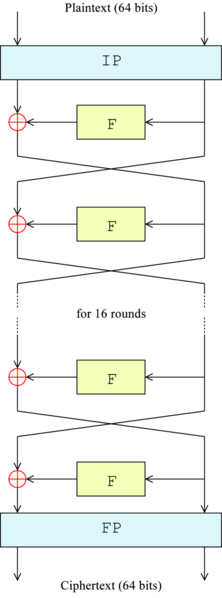
\includegraphics[scale=0.6]{immagini/DES_fastell.png}
\end{figure}

\subsubsection{La funzione Feistell}

\begin{figure}[htbp]
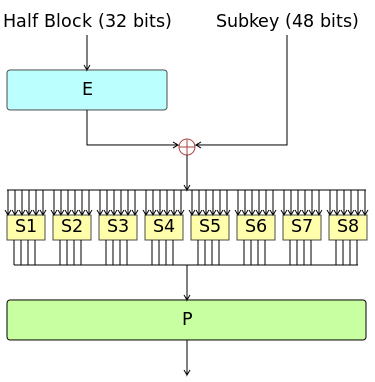
\includegraphics[scale=0.6]{immagini/DES_round.png}
\end{figure}

La funzione Feistel, opera su mezzo blocco (32 bit) per volta e consiste di 4 passi:
\begin{itemize}
\item  Espansione - il mezzo blocco di 32 bit è espanso fino a 48 bit utilizzando la permutazione di espansione contraddistinta con E nello schema, che duplica alcuni bit.
\item Miscelazione con la chiave - il risultato è combinato con una sottochiave usando un'operazione di XOR. Sedici sottochiavi di 48 bit, una per ogni ciclo, sono derivate dalla chiave principale usando il gestore della chiave (descritto più avanti).
\item Sostituzione - dopo la miscelazione con la sottochiave, il blocco viene diviso in 8 parti di 6 bit prima del processamento con le S-box o substitution box (scatole di sostituzione). Ognuna delle 8 S-box sostituisce 6 bit in input con 4 bit in output mediante una trasformazione non lineare effettuata attraverso una tabella. Le S-box forniscono il cuore della sicurezza del DES — senza di esse, la cifratura sarebbe lineare e quindi facilmente violabile.
\item Permutazione - infine, i 32 bit risultanti dalle S-box sono riordinati in base alle permutazioni fisse della P-box o permutation box.  
\end{itemize}

L'alternanza di sostituzioni mediante le S-box, le permutazioni con la P-box e le espansioni forniscono la cosiddetta confusione e diffusione, un concetto identificato da Claude Shannon negli anni quaranta come condizione necessaria per rendere pratica e sicura la cifratura.

\subsubsection{Gestore della chiave}

\begin{figure}[htbp]
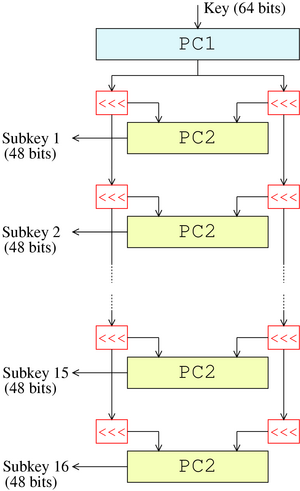
\includegraphics[scale=0.6]{immagini/DES_gestore_chiave.png}
\end{figure}

L'algoritmo che genera le sottochiavi. Inizialmente, vengono selezionati 56 bit della chiave dagli iniziali 64 bit mediante la funzione Permuted Choice 1 (PC-1) - i rimanenti 8 bit sono scartati o utilizzati come bit di controllo della parità. I 56 vengono poi suddivisi in 2 metà di 28 bit; ogni metà è poi trattata separatamente. Nei cicli successivi entrambe le metà vengono fatte slittare verso sinistra di 1 o 2 bit (per i round 1, 2, 9, 16 lo shift, cioè lo slittamento, è di 1 bit, per gli altri è di 2) e quindi vengono scelti 48 bit per la sottochiave mediante la funzione Permuted Choice 2 (PC-2) - 24 bit dalla metà di sinistra e 24 bit da quella di destra. La rotazione (denotata da "<<<" nello schema) significa che in ogni sottochiave è usato un insieme differente di bit; ogni bit è usato più o meno in 14 delle 16 sottochiavi.Il gestore delle chiavi per la decifratura è simile - deve generare le chiavi nell'ordine inverso quindi la rotazione è verso destra invece che verso sinistra.

\subsection{Attacco a DES}
\subsubsection{prefazione}
In questo corso si vede l'attacco a DES in una versione semplificata: i Round sono 3 anzichè 16, l'input è formato da blocchi di 12 bit e di 6 bit per blocco, la funzione di espansione porta da 6 a 8 bit e le sbox prendono 4 bit in input e 3 in output. In questo modo l'attacco a DES è deterministico mentre nella versione completa di DES questo attacco è probabilistico.

\section{Modalità di funzionamento dei cifrari a blocchi}
\subsection{prefazione}
Le modalità di funzionamento dei cifrari a blocchi sono state definite inizialmente dal NIST (National Institute of Standards and Technology) nel documento FIPS 81 (Federal Information Processing Standard) intitolato "DES modes of operation" affinché l'algoritmo di cifratura DES potesse essere applicato ad una varietà di situazioni differenti.
Queste modalità cercano dunque di considerare tutte le possibili applicazioni della crittografia per cui può essere utilizzato l'algoritmo DES; con la successiva comparsa di nuovi requisiti, il NIST ha espanso l'elenco delle modalità di funzionamento a cinque, nel documento Special Publication 800-38A.
Tali modalità possono essere utilizzate con qualsiasi algoritmo di cifratura simmetrica a blocchi, tra cui Triple DES e AES.
\subsection{ECB (eletronic codebook}
La modalità ECB è la più semplice. Il testo in chiaro viene gestito 64 bit per volta; ognuno dei blocchi di 64 bit viene cifrato con la stessa chiave. Per messaggi più lunghi di 64 bit, si procede suddividendo il messaggio in blocchi di 64 bit, utilizzando, se necessario, bit di riempimento nell'ultimo blocco.

\begin{figure}[htbp]
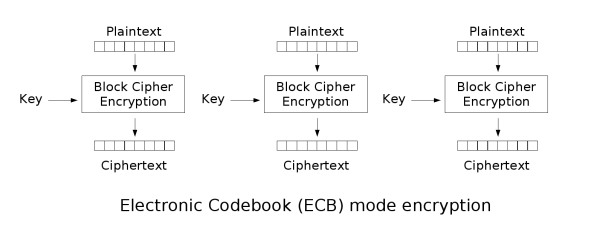
\includegraphics[scale=0.6]{immagini/ecb.png}
\end{figure}

Per una data chiave, esiste un unico testo cifrato per ogni blocco di testo in chiaro di 64 bit; in altre parole, se nel messaggio compare più volte lo stesso blocco di 64 bit di testo in chiaro, verrà prodotto sempre lo stesso testo cifrato. Per questo motivo, il metodo ECB è ideale per limitati volumi di dati (ad esempio, la trasmissione di una chiave di cifratura), poiché per messaggi più lunghi potrebbe essere insicuro: se si trattasse di dover cifrare un messaggio molto strutturato, l'analisi crittografica potrebbe sfruttarne le regolarità.

\subsection{Cipher block chain}
Per superare i limiti di sicurezza di ECB, è necessario l'utilizzo di una tecnica in cui lo stesso blocco di testo in chiaro, se ripetuto, produce blocchi di testo cifrato differenti. Questo è ciò che accade con la modalità CBC, in cui l'input dell'algoritmo di crittografia è il risultato dello XOR tra il blocco di testo in chiaro corrente e il blocco di testo cifrato precedente; per ciascun blocco viene utilizzata la stessa chiave.
In fase di decifratura, ciascun blocco di testo cifrato passa attraverso l'algoritmo di decrittografia; il risultato subisce uno XOR con il blocco di testo cifrato precedente, per produrre il blocco di testo in chiaro.

\begin{figure}[htbp]
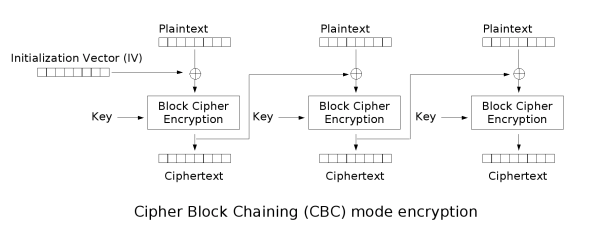
\includegraphics[scale=0.8]{immagini/cbc.png}
\end{figure}

Per produrre il primo blocco di testo cifrato, lo XOR viene effettuato tra un vettore di inizializzazione IV (dall'inglese initialization vector) e il primo blocco di testo in chiaro. In decifratura, l'IV subisce uno XOR con l'output dell'algoritmo di decrittografia in modo da ottenere nuovamente il primo blocco di testo in chiaro.
Il vettore di inizializzazione IV deve essere dunque noto non solo al mittente ma anche al destinatario, che tipicamente lo riceve assieme alla chiave; entrambi i valori vengono crittati in modalità ECB.
In conclusione, questa modalità è la più appropriata per cifrare messaggi più lunghi di 64 bit. Inoltre, la modalità CBC può essere utilizzata anche per l'autenticazione.

\subsection{Cipher Feedback (CFB)}
La modalità CFB è stata ideata per convertire idealmente una cifratura a blocchi in una cifratura a flusso. La cifratura a flussi non necessita di eseguire riempimenti e può inoltre operare in tempo reale.
Nell'operazione di cifratura, l'input della funzione di crittografia è un registro a scorrimento a 64 bit che inizialmente viene impostato con un vettore di inizializzazione IV (Initialization Vector). Gli s bit più significativi (ovvero quelli più a sinistra) dell'output subiscono uno XOR con il primo segmento di testo in chiaro P1 per produrre la prima unità di testo cifrato C1. Il contenuto del registro di scorrimento viene fatto scorrere a sinistra di s bit, e negli s bit meno significativi (quelli più a destra) del registro viene inserito C1. Il processo viene reiterato fino all'esaurimento di tutte le unità di testo in chiaro.
All'atto della decifratura, si utilizza il medesimo schema, tranne per il fatto che le unità di testo cifrato ricevute sono sottoposte ad uno XOR con l'output della funzione di crittografia. Non si utilizza dunque la funzione di decrittografia, perché, se SS(X) sono gli s bit più significativi di X, allora:
$$ C_1 = P_1 \oplus S_S(E_k(IV)) $$\\
Quindi:\\
$$ P_1 = C_1 \oplus S_S(E_k(IV)) $$\\
e lo stesso ragionamento vale per i passi successivi.


\begin{figure}[htbp]
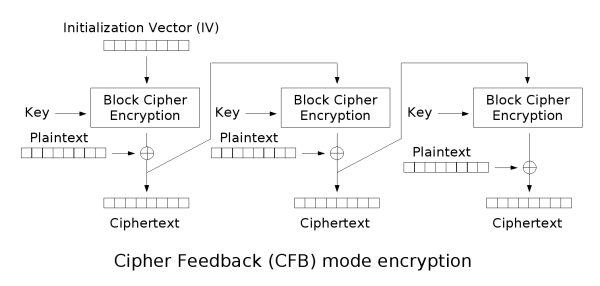
\includegraphics[scale=0.8]{immagini/cfb.png}
\end{figure}

Il problema di questa tecnica di cifratura risulta nella facilità della propagazione dell'errore dato che al passo $k_i$ la corretta decifratura dipende dal passo $k_{i-1}$.

\subsection{Output Feedback (OFB)}
La modalità OFB è molto simile alla CFB. Il vantaggio della OFB è che non propaga gli errori di trasmissione dei bit. Il suo svantaggio è che è più vulnerabile a un attacco a modifica del flusso dei messaggi.

\begin{figure}[htbp]
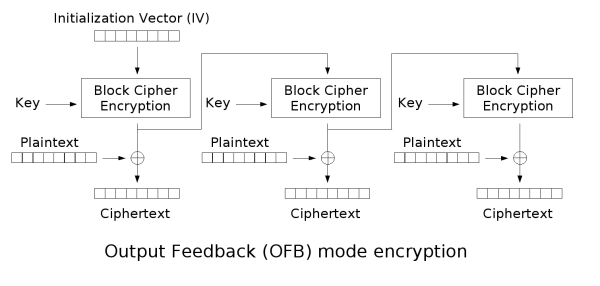
\includegraphics[scale=0.8]{immagini/ofb.png}
\end{figure}

Solitamente si usa questa modalità quando si può accettare un ritardo nella risposta rispetto alla sua correttezza

\subsection{Counter (CTR)}
uesta quinta modalità è stata introdotta successivamente alle altre quattro, per poter essere applicata a ATM (Asynchronous Transfer Mode) e a IPsec (IP security).
In questa modalità viene utilizzato un contatore corrispondente alle dimensioni del blocco di testo in chiaro. Il requisito essenziale è che il suo valore sia differente per ciascun blocco da cifrare; in genere viene inizializzato con un determinato valore e poi incrementato di un'unità per ogni blocco successivo (modulo $2?b$ dove $b$ corrisponde alle dimensioni del blocco).
Per la cifratura, il contatore viene crittografato e poi si applica uno XOR col blocco di testo in chiaro per produrre il blocco di testo cifrato.
Per la decifratura si utilizza la stessa sequenza di valori del contatore ai quali si applica lo XOR con i blocchi di testo cifrato.

\begin{figure}[htbp]
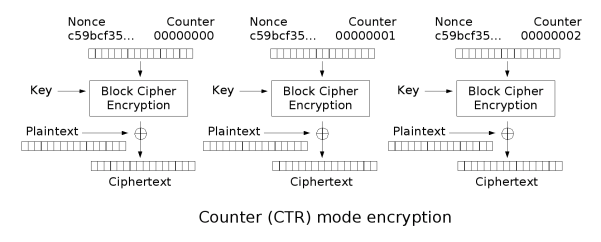
\includegraphics[scale=0.8]{immagini/ctr.png}
\end{figure}

I vantaggi della modalità CTR sono:
\begin{itemize}
\item efficienza dell'hardware;
\item efficienza del software;
\item pre-elaborazioni;
\item accesso diretto;
\item sicurezza dimostrabile;
\item semplicità.
\end{itemize}
    
\section{Problema del logaritmo discreto}
Il calcolo dei logaritmi discreti sembra un problema difficile (non sono noti algoritmi efficienti), mentre il problema inverso dell'esponenziazione discreta non lo è. Quest'asimmetria è analoga a quella fra la fattorizzazione di interi e la moltiplicazione di interi. Entrambe queste asimmetrie sono state utilizzate per la costruzione di sistemi crittografici. Nella crittografia basata sui logaritmi discreti scelte comuni per il gruppo G sono i gruppi ciclici $\mathbb{Z}_p^*$. Le più recenti applicazioni della crittografia usano i logaritmi discreti in sottogruppi ciclici di curve ellittiche su campi finiti; vediamo ora la effettiva difficoltà di riottenere il plaintext (che sarà indicato con x) dato il ciphertext (che sarà indicato con b). Abbiamo quindi, formalmente, il seguente problema:

$$ a^x=b\mod(p)$$ con p primo.\\

Come posso attaccarlo? Sfruttando il piccolo teorema di Fermat che ci dice $a^{p-1} \equiv 1 \mod(p)$ e $a^{\phi(n)}\equiv 1 \mod(n)$. Riscriviamo il problema come:\\

$$ \alpha^x=\beta\mod(p)$$ con p primo e $\alpha,\beta \in Z_p$\\

Vogliamo inoltre che $\alpha$ sia una \textit{radice primitiva} di $Z_p$ ovvero che se $\alpha$ è elevato a tutte le classi di resto di $Z_p$ allora genera tutto il campo una e una sola volta.\\
Esempio:\\
$
\alpha = 3
\\Z_p=\{0,1,2,3,4,5,6\}\\
\alpha^1 = 3\\
\alpha^2 = 2\\
\alpha^3 = 6\\
\alpha^4 = 4\\
\alpha^5 = 5\\
\alpha^6 = 1\\
$
Quindi nel nostro esempio 3 è una radice primitiva. Tornando al caso generale per il piccolo teorema di Fermat sappiamo che $\alpha^{p-1}\equiv 1 \mod(p)$ quindi:
$$ \alpha^{(p-1)\cdot 1}\equiv 1 \mod(p) =\alpha^{(p-1)\cdot \frac{2}{2}}\equiv 1 \mod(p) = (\alpha^{\frac{p-1}{2}})^\frac{1}{2}\equiv 1 \mod(p) =$$ $$ (\alpha^{\frac{p-1}{2}})^x\equiv 1 \mod(p) = 1 \vee -1 $$
arrivati alla fine possiamo dire che il valore $1$ non è accettabile perchè sappiamo che $\alpha$ è una radice primitiva e che $\alpha^{p-1}\equiv 1 \mod(p)$. Quindi l'unico valore accettabile è $-1$, proseguiamo riprendendo il problema:\\
$$ (\alpha^{\frac{p-1}{2}})^x\equiv \beta^{\frac{p-1}{2}} $$\\

sappiamo che $\alpha = -1$ quindi:\\

$$(-1)^x \equiv \beta^{\frac{p-1}{2}}$$

Quindi facendo così posso capire se x è pari o dispari ma ho ancora uno spazio delle chiavi ancora troppo grande! Infatti se lo spazio delle chiavi è $2^{300}$ l'ho ridotto a $2^{299}$. Questa tecnica non è molto efficente, vediamo ora una versione più evoluta: l'attacco baby step - giant step.

\subsection{Attacco baby step - giant step}

$\alpha^x \equiv \beta \mod(p)$ - $N^2\ge p-1 $ - $N=\mathcal{b} \sqrt{p-1} \mathcal{c} +1$\\

Ora creo una lista di potenze di $\alpha$ in questo modo: $\sum_{J=0}^{J=N} \alpha^J$ e successivamente inizio a generare la lista $\beta \cdot \alpha^{-N\cdot K}$ con $0 \leq k \leq N$ fino a quando o non si raggiunge $\alpha^J$ oppure non si trova $\alpha^n \equiv \beta \cdot\alpha^{-N\cdot k}$, se trovo quel valore allora posso sfruttare Fermat, infatti:
$\alpha^n \equiv \beta \cdot\alpha^{-N\cdot k} \Rightarrow \alpha^n \cdot \alpha^{-N\cdot k} \equiv \beta \Rightarrow \alpha^{j+N\cdot k} \equiv \beta $\\

Ma $j+N\cdot k$ è il valore x che stavamo cercando. Questo attacco va bene fino a $10^20$ cifre poi il tempo di computazione diventa troppo elevato.

\subsection{Attacco Index Calculus}
Questo tipo di attacco esegue una precomputazione "sperando" che con i conti fatti si possa trovare la il valore di x. Eva recupera il messaggio cifrato $\beta=\alpha^x$ la base $\alpha$ e il numero primo della chiave pubblica. A questo punto Eva sceglie una base di fattorizzazione ovvero un insieme di numeri primi minori di un valore N. A questo punto trovo un po' di valori $\alpha^k$ con $0\leq k \leq \beta$ e se riesco a trovare il valore congruo in $Z_p$ esprimibile tramite la base di fattorizazione tengo il valore altrimenti calcolo altri $\alpha^k$ fino a quando non ho trovato tutti i valori che posso rappresentare tramite la base di fattorizzazione in $Z_p$. A questo punto calcolo i vari logaritmi dei valori che ho trovatoè, finiti questi calcoli genero un valore $r$ casuale e calcolo $\beta\cdot\alpha^r$ se questo valore posso rappresentarlo tramite la base di fattorizzazione allora posso trovare il valore x, infatti:
$$ \beta \cdot \alpha^r =
 \alpha^x \cdot \alpha^r = 
 \log_{\alpha}(\alpha^x \cdot \alpha^r) =
  \log_{\alpha}(\alpha^{x+r})) = x+r$$\\

A questo punto basta sottrare $r$ al valore ottenuto e si riesce ad ottenere x, se invece non si riesce ad ottenere $\beta\cdot\alpha^r$ con la base di fattorizzazione devo provare con un altro $r$.
\section{Lo scambio di chiavi di Diffie ed Helman}
Sfruttando il logaritmo discreto Diffie ed Helman hanno sviluppato una tecnica di scambio delle chiavi senza che queste ultime passino effettivamente sul canale, per capire il funzionamento facciamo un esempio: Alice e Bob lavorano per la stessa azienda di colori, hanno deciso che per sicurezza dovranno usare un particolare inchiostro colorato per scrivere le lettere che si scambiano, il loro problema è come possano spedirsi i colori senza che Eva (la concorrente) possa guardare e copiare l'inchiostro. Il seguete schema spiega il funzionamento:
\begin{figure}[htbp]
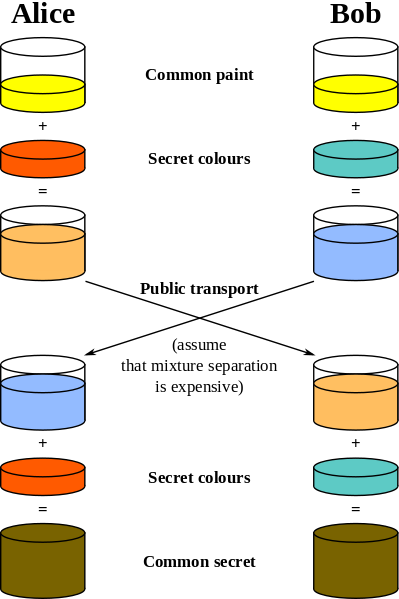
\includegraphics[scale=0.6]{immagini/scambioChiavi.png}
\end{figure}

Nella pratica Alice comunica a Bob due valori $\alpha$ e $p$ successivamente sia Alice che Bob calcolano ognuno un valore $x$ nel caso di Alice e $y$ nel caso di Bob successivamente fanno rispettivamente  $\alpha^x$ e $\alpha^y$ e si scambiano il risultato, successivamente Alice farà $(\alpha^y)^x$ e Bob invece $(\alpha^x)^y$ grazie al problema del logaritmo discreto sappiamo che eva non riuscirà ad ottenere i due numeri segreti $x,y$ quindi Alice e Bob possono comunicare in sicurezza le loro informazioni.

\section{Cifrario di Elgamal}
ElGamal è un sistema di cifratura a chiave pubblica, proposto dal ricercatore egiziano-americano Taher Elgamal nel 1985. Lo schema è basato sulla difficoltà del calcolo del logaritmo discreto.Ci sono tre fasi in questo algoritmo:
\begin{itemize}
\item[1] Alice genera e rende nota una chiave pubblica:$Y_{Alice} = (\alpha^{X_{Alice}} \bmod p)$, analogamente Bob genera la sua chiave pubblica:$Y_{Bob} = (\alpha^{X_{Bob}} \bmod p)$ dove:
\begin{itemize}
\item p è numero primo grande
\item $\alpha$ radice primitiva di p
\item $a$ scelto a caso in maniera uniforme tra $[1,(q-1)]$, che costituisce la chiave privata di Alice e deve essere mantenuto segreto.
\item $b$ scelto a caso in maniera uniforme tra $[1,(q-1)]$, che costituisce la chiave privata di Bob e deve essere mantenuto segreto.
\end{itemize} 
\item[2] Alice vuole inviare un messaggio a Bob, Bob rende disponibile la sua chiave pubblica composta da (p,$\alpha$,$\beta$) dove $\beta = \alpha^b \mod(p)$. Alice recupera queste informazioni e genera $r=\alpha^k\mod p$ e $t=\beta\cdot m \mod(p)$.
\item[3] Il testo cifrato (r,t) viene inviato a Bob il quale recupera M nel seguente modo: $t\cdot r^b \mod(p) \equiv m$ 
\end{itemize}

Il procedimento è matematicamente corretto perchè:\\
$t\cdot r^{-b}=(\beta^k\cdot m)\cdot(\alpha^k)^{-b}=((\alpha^b)^{k}\cdot m)\cdot(\alpha^k)^{-b} = 1 \cdot m$

\subsection{Problematiche di Elgamal}
Uno sbadato Bob potrebbe usare $b$ per due diversi M, Eva se ne accorge perchè vengono spedite due messaggi con $r$ uguale quindi (Se Eva può fare un attacco Know plaintext):
$$ \frac{t_1}{M_1}=\beta_k=\frac{t_2}{m_2} \Rightarrow \frac{t_1}{m_1\cdot t_2} = \frac{1}{m_2} $$

\section{Bit Commitment}
Si utilizza il Bit commitment nel momento in cui Alice vuole rassicurare Bob che ha una informazione senza dare a Bob quest'ultima. Anche in questo caso sfrutto il logaritmo discreto. Scelgo $p,\alpha$ e $x$ dove $x$ è la nostra informazione, poi spedisco $\beta = \alpha^x \mod(p)$ come prova


%ho due casi:\\
%\begin{center}
%$\begin{cases}
%MCD(p,m) \not= 1\\
%MCD(p,m) = 1
%\end{cases}
%$\\
%\end{center}

\end{document}

